\documentclass[tikz,11pt,border=10pt]{standalone}
%\documentclass[a4paper]{article}

\usepackage{pgfplots}
\usepgfplotslibrary{polar}
\usepackage{tikz}
\usetikzlibrary{shapes,arrows}

\usepackage{pgfplots}
\pgfplotsset{/pgf/number format/use comma,compat=newest}

\begin{document}

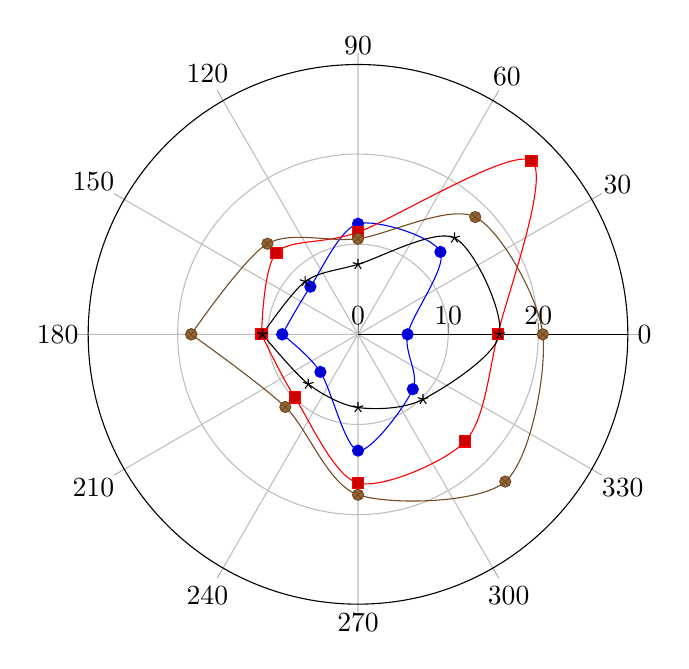
\begin{tikzpicture}
\begin{polaraxis}
[smooth]
\addplot coordinates
{(0, -8.4) (45, -5.9) (90, -12.9) (135, -8.6) (180, -5.5)
 (225, -12.93) (270, -12.27) (315, -7.47) (360, -8.4)};
 \addplot coordinates
{(0, -10.7) (45, -9.9) (90, -16.5) (135, -16.8) (180, -15.5)
 (225, -27.21) (270, -11.33) (315, -12.8) (360, -10.7)};
\addplot coordinates
{(0, -18.5) (45, -11.4) (90, -17.8) (135, -23.1) (180, -20.5)
 (225, -18.4) (270, -10.6) (315, -14.21) (360, -18.5)};
 \addplot coordinates
{(0, -10.6) (45, -7.8) (90, -8.12) (135, -10.20) (180, -15.7)
 (225, -15.13) (270, -7.76) (315, -8.29) (360, -10.6)};
\end{polaraxis}
\end{tikzpicture}

\end{document}